\title{Combinational Design}
\begin{document}
\section{Documentation}

\begin{frame}{Documentation types}
  \begin{itemize}
    \item Specification
    \item Block diagram
    \item Schematic diagram
    \item Timing diagram
    \item Sturctured logic device description
    \item Circuit description
  \end{itemize}
\end{frame}

Often your testing tools (testbenches, etc.) are a good starting point for documentation.

\subsection{Block Diagrams}

\begin{frame}{Block diagrams}
  \begin{definition}
    A \alert{block diagram} shows the inputs, outputs, functional modules, and internal data flow of a system.
  \end{definition}
  Block diagram tips:
  \begin{itemize}
    \item Specify signal or bus names.
    \item Specify signal directions.
    \item If it looks too complicated, it probably is.  Abstract a complex section into a single block.
  \end{itemize}
\end{frame}

\begin{frame}{Motorola 6800 block diagram}
  \begin{center}
    \includegraphics[scale=0.4]{6800_block_diagram.jpg}
  \end{center}
\end{frame}

\begin{frame}{Intel Core i7 block diagram}
  \begin{center}
    \includegraphics[scale=0.4]{core_i7_block_diagram.jpg}
  \end{center}
\end{frame}

\subsection{Active Levels}

\begin{frame}{Active levels for signal}
  Previously, we discussed positive (active high) and negative (active low) logic.
  \begin{block}{Signal Active Levels}
    Even if a given circuit uses, for exmaple, positive logic, some signals may be \alert{active low}.  There names usually indicate this:
    \begin{itemize}
      \item RESET-
      \item ERROR.L
      \item ENABLE*
      \item TRANSMIT\_L
    \end{itemize}
  \end{block}
\end{frame}

These different active levels are usually the result of NAND and NOR logic gates being cheaper and faster than AND and OR logic gates.

\begin{frame}{Active levels on pins}
  Pins on an IC may be active low inputs or outputs.  They are usually indicated like this.\\
  \begin{center}
    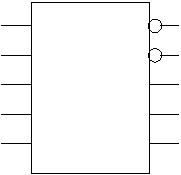
\includegraphics{ActiveLowIC}
  \end{center}
\end{frame}

\subsection{Buses}

\begin{frame}{If this bus goes below 60 mph...}
  \begin{definition}
    A \alert{bus} is a collection of two or more signals that are related.  It is usually drawn with a thicker line on a schematic diagram.
  \end{definition}
  Some examples of common buses include:
  \begin{itemize}
    \item ADDR[15:0] - A 16-bit address bus
    \item DATA[31:0] - A 32-bit data bus
    \item CONTROL - A collection of various control signals.
  \end{itemize}
  Busses are used to simplify documentation.  In the physical circuit, all of the signals are separate traces.
\end{frame}

\section{Circuit Timing}

\subsection{Timing Diagrams}

\begin{frame}{Timing Diagrams}
  The timing diagram for a circuit specifies the interaction between the signals.\\
  \begin{center}
    \includegraphics[scale=0.7]{TimingDiagram}
  \end{center}
\end{frame}

\begin{frame}{Progagation delay}
  \begin{block}{Propagation Delay}
    The time required for the inputs to produce outputs can vary in circuit.  It is usually specified in terms of its
    \begin{itemize}
      \item Minimum value
      \item Typical value
      \item Maximum value
    \end{itemize}
  \end{block}
\end{frame}

\section{Combinational PLDs}

\subsection{Programmable Logic Arrays}

\begin{frame}{Programmable logic arrays}
  Programmable logic arrays (PLA) are the simplest type of PLD.
  \begin{itemize}
    \item They consist of an AND-OR configuration with each input and its complement available.
    \item A give PLA can accept a number of inputs ($n$), outputs ($m$) and product terms ($p$).
    \item Programmable fuses are used to connect the inputs to the AND gates and the AND gates to the OR gates.
  \end{itemize}
\end{frame}

An example is on pg 371 of the text.

\subsection{Programmable Array Logic}

\begin{frame}{Programmable array logic}
  Programmable array logic (PAL) devices use a fixed OR array, where a set of AND gates always feed another set of OR gates.
  \begin{itemize}
    \item These devices can enable or disable a given output.
    \item A number of the outputs can also be used as inputs.
  \end{itemize}
\end{frame}

An example is on pg 375 of the text.

\subsection{General Array Logic}

\begin{frame}{General array logic}
  General array logic (GAL) is another type of AND-OR array.
  \begin{itemize}
    \item GAL devices contain an additional XOR gate on each pin output that can be used to invert that output.
    \item Often the inverse of a logic function will be simpler than the actual function, so this XOR gate is used to invert all of the outputs.
  \end{itemize}
\end{frame}

\subsection {Complex Programmable Logic}

\begin{frame}{Complex programmable logic}
  Complex programmable logic devices (CPLD) are simply collections of multuple PLDs.
  \begin{itemize}
    \item A \alert{fitter} program is often used to determine how best to program a logic function into a CPLD.
    \item Usually, the user can provide constraints to the fitter to allow it to work more effectively.
  \end{itemize}
\end{frame}

\end{document}
